\section{Gravity assist analysis}
\label{sec:gravity-assist-analysis}

Gravity assists are a well-known maneuver for changing the velocity of a
spacecraft by using the gravitational pull of a planet. The spacecraft flies by
the planet and gains or loses velocity depending on the relative motion of the
planet and the spacecraft. This technique is used to save fuel and time, and is
commonly used in interplanetary missions. \cite{flandro1966} makes a great
introduction about the basics of gravity assists that lead to the development of
missions like Voyayer I and Voyayer II.

This analysis only considers unpowered gravity assists, in which the spacecraft
does not lose mass or performs any propulsive maneuvers.

%\subsection{Revisiting gravity assists}

The characteristic energy of a spacecraft in the heliocentric frame is given by
equation \ref{eq:helio-energy}:

\begin{equation}
  E_{\Sun} = \frac{1}{2}V_{\Sun}^2
  \label{eq:helio-energy}
\end{equation}

where $V_{\Sun}$ is the velocity of the spacecraft in the heliocentric frame.

Consider a planet moving at a speed of $V_p$ in the heliocentric frame. Assuming
a spacecraft approaches the planet with a speed of $\vec{v}_{\text{in,}\infty}$
and that it leaves the planet with a speed of $\vec{v}_{\text{out,}\infty}$,
both as seen by the planet. From the point of view of the planet,
$v_{\text{in,}\infty} = v_{\text{out,}\infty} = v_{\infty}$. Despite their
modulus being the same, the direction of these vectors is different. Thus,
$\vec{v}_{\text{in,}\infty} \neq \vec{v}_{\text{out,}\infty}$.

From the heliocentric perspective, the spacecraft approaches the planet with a
velocity $\vec{V}_{\text{in}} = \vec{V_p} + \vec{v}_{\text{in,}\infty}$ and
leaves the planet with a velocity $\vec{V}_{\text{out}} = V_p +
  \vec{v}_{\text{out,}\infty}$.

The angle between $\vec{v}_{\text{in,}\infty}$ and $\vec{v}_{\text{out,}\infty}$
is known as the deflection angle, $\psi$. The speed $v){\infty}$ and the maximum
$\psi$ are related once the altitude $h = d - R_p$ of the flyby is set, being
$R_p$ the radius of the planet. This relation is exposed by equation
\ref{eq:max-deflection-angle}:

\begin{equation}
  \psi_{\max} = 2 \cdot \arcsin{\left(\frac{\mu}{\mu + {v}^{2}_{\infty}(R_p + h)}\right)}
  \label{eq:max-deflection-angle}
\end{equation}

Figure \ref{fig:deflection-angle-at-speed} is generated by solving equation
\ref{eq:max-deflection-angle} at an altitude of $h = R_p$ for different values
of $v_{\infty}$ at each planet of the solar system.

\begin{figure}[H]
  \centering
  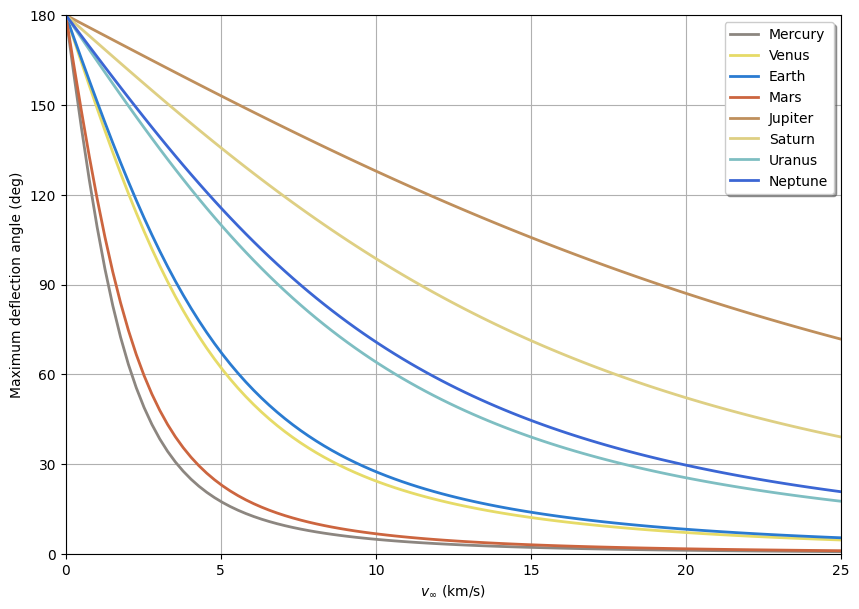
\includegraphics[width=0.9\textwidth]{fig/static/deflection_angle.png}
  \caption[Maximum deflection angle as a function of the speed of the spacecraft
    at different planets.]{Maximum deflection angle as a function of the
    speed of the spacecraft at different planets. Flyby altitude is
    $h = R_p$.}
  \label{fig:deflection-angle-at-speed}
\end{figure}

\begin{figure}[H]
  \centering
  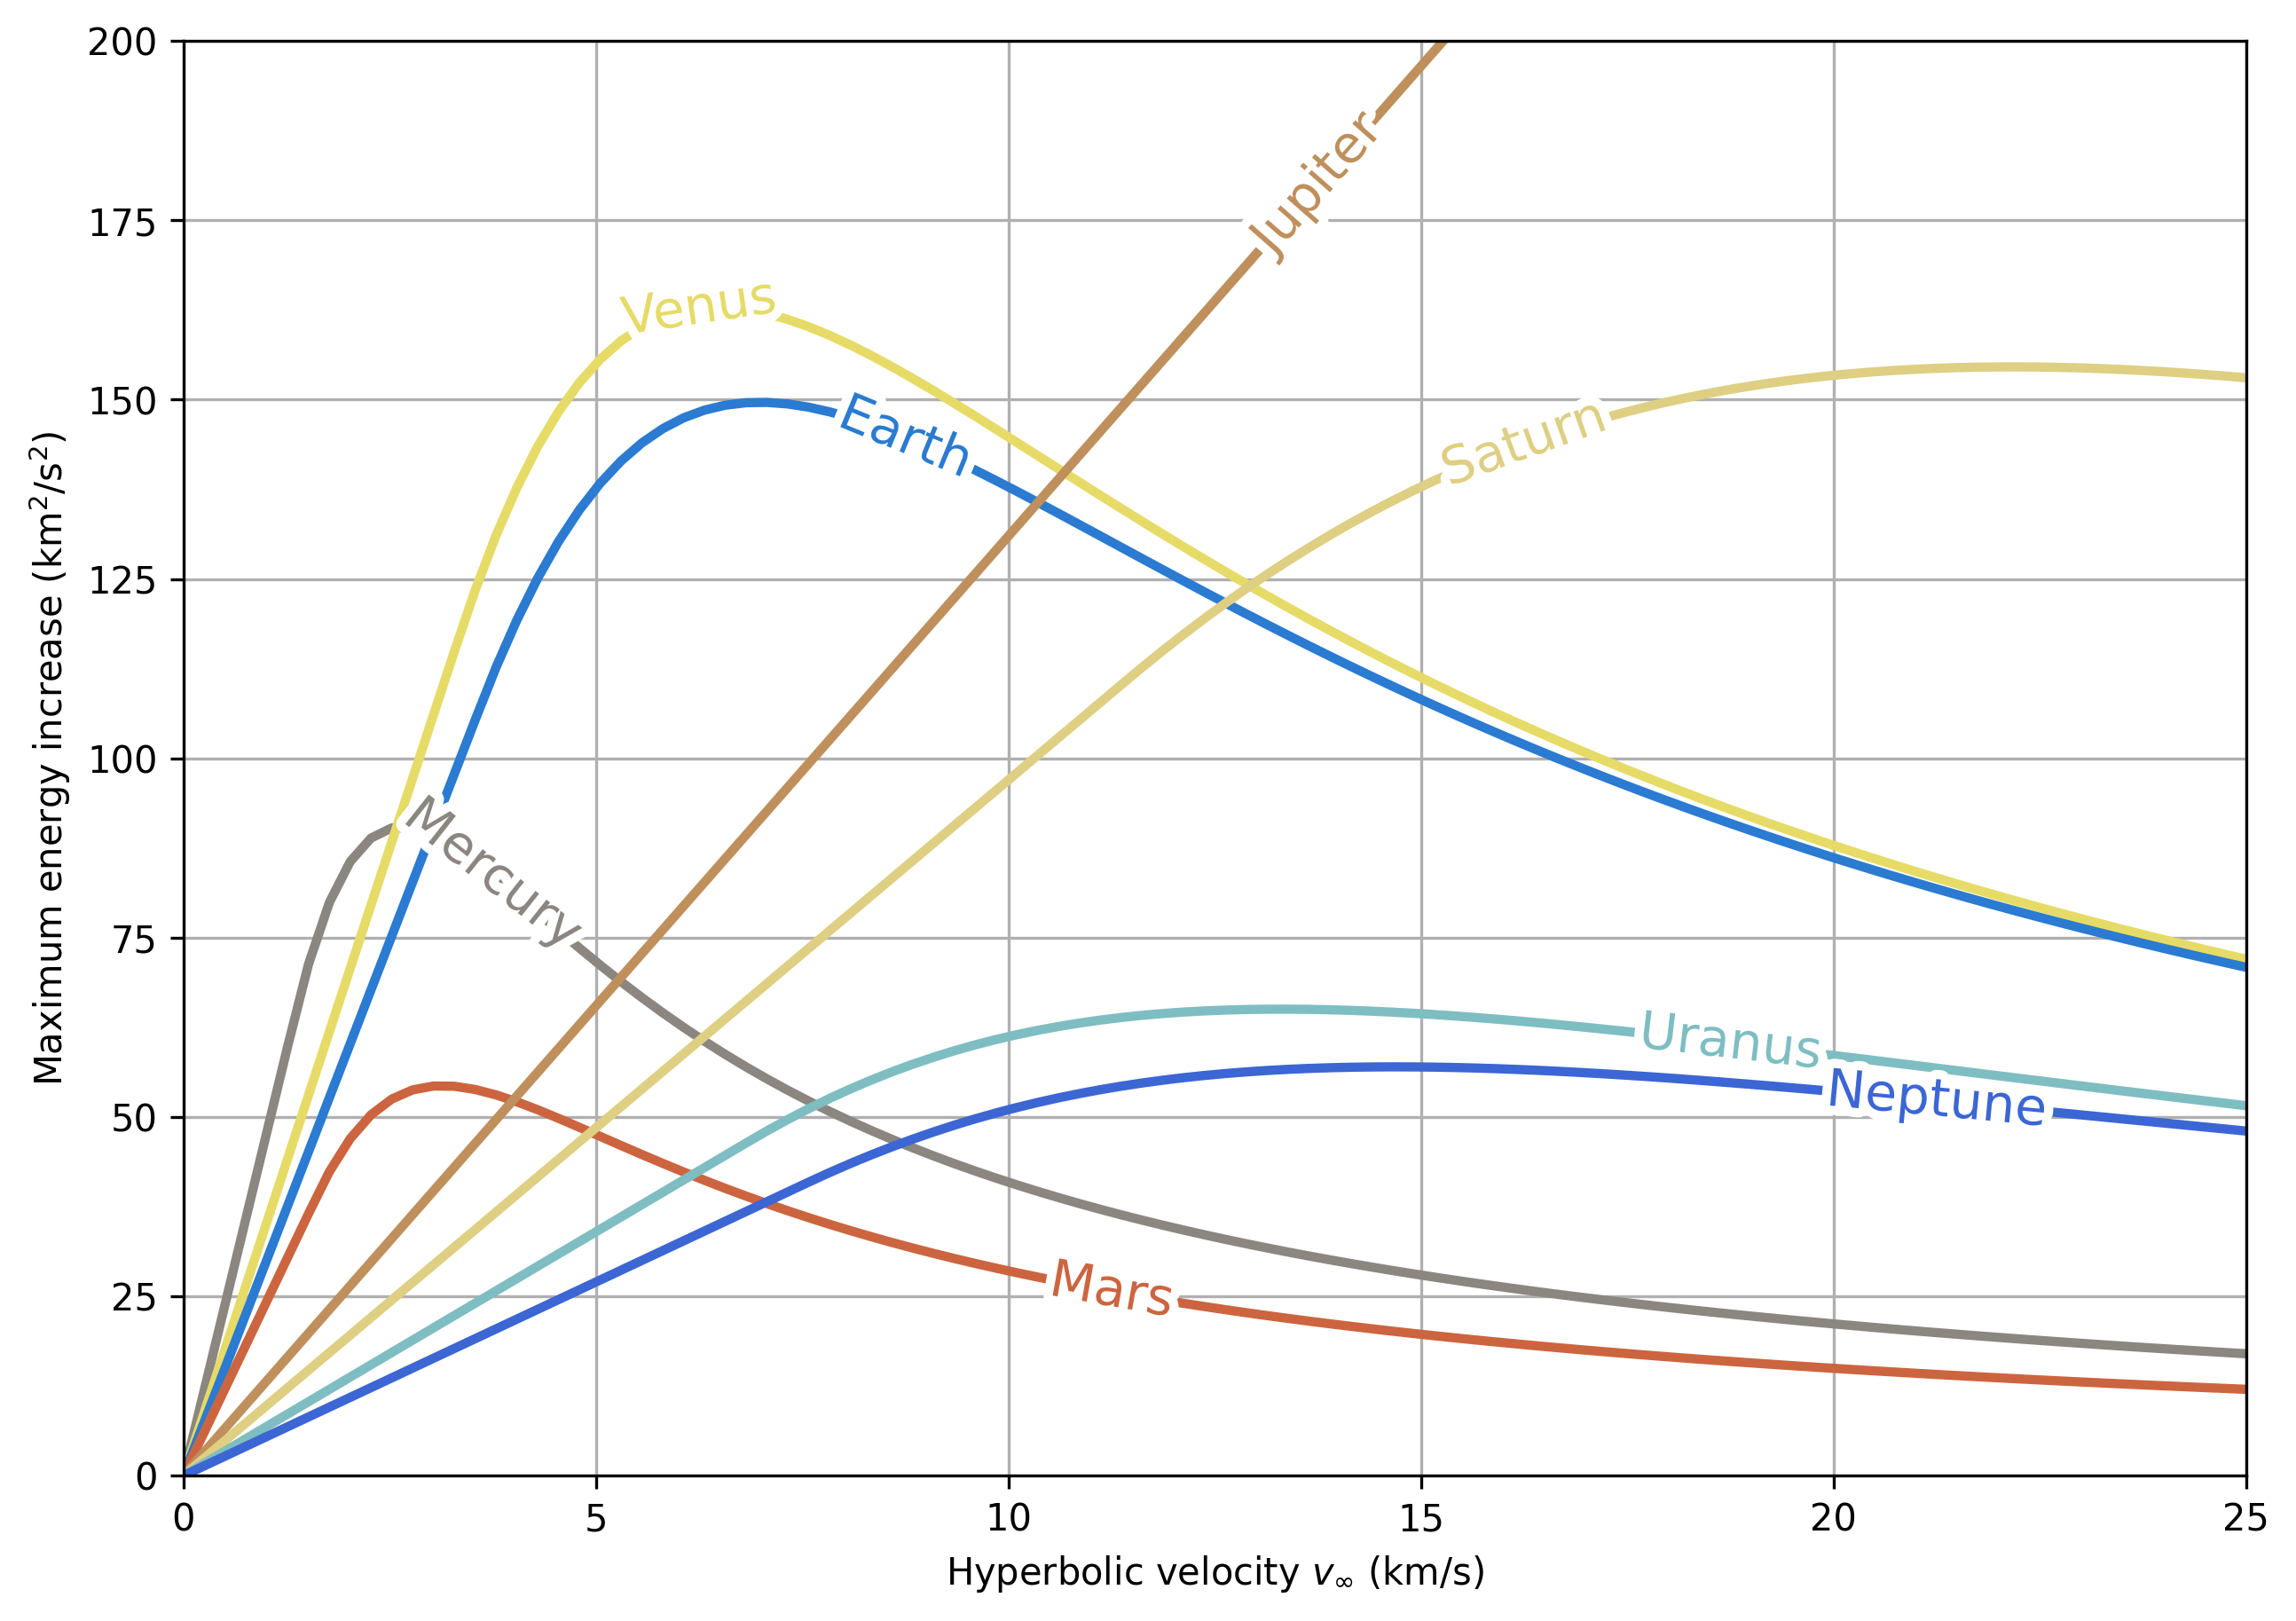
\includegraphics[width=0.9\textwidth]{fig/static/max_energy.png}
  \caption[Maximum energy increment as a function of the speed of the
    spacecraft at different planets.]{Maximum energy increment as a function
    of the speed of the spacecraft at different planets. Evaluated at the
    maximum deflection angle. Mean values for planetary orbital speed were used.}
  \label{fig:max-energy-at-speed}
\end{figure}

Looking at figure \ref{fig:deflection-angle-at-speed}, one could think that
Jupiter woudl provide the highest increments in the characteristic energy since
it provides the highest deflection angle for a given hyperbolic speed. However,
figure \ref{fig:max-energy-at-speed} shows that the maximum energy increment
depends on the planet.

The relationship between the increment in the characteristic energy and the
hyperbolic speed is not linear and is given by equation
\ref{eq:energy-increment}:

\begin{equation}
  \Delta E = f_{\text{max}} E^{\ast} = f_{\text{max}} V_p v_{\infty}
  \label{eq:energy-increment}
\end{equation}

where $f_{\text{max}}$ is the maximum energy increment factor given by equation
\ref{eq:max-energy-increment-factor}:

\begin{equation}
  f_{\text{max}} = \begin{cases}
    \frac{\cos{\epsilon} + 1}{2}                                         & \text{if } \epsilon \geq \pi - \psi_{\max} \\
    \frac{\cos{\epsilon} - \cos{\left(\psi_{\max} + \epsilon\right)}}{2} & \text{otherwise}
  \end{cases}
  \label{eq:max-energy-increment-factor}
\end{equation}

where $\epsilon$ is the angle between the direction of the asymptote and the
planet's velocity vector.

Note that for a certain hyperbolic speed, the maximum energy other planets
rather than Jupiter may provide higher energy increments. For example, below
$v_{\infty} < 10$ km/s, Venus and Earth are more efficient than Jupiter for
$\psi_{\text{max}}$. The same happens for Mercury at $v_{\text{max}} < 5.00$
km/s.

Despite this analysis, it is important to note that the energy increment does
not always take place at the maximum deflection angle. The orientation of the
incoming hyperbolic speed vector and its magnitude will determine the state
after the gravity assist. In fact, it may be possible that a gravity assist is
not beneficial at all, requiring more fuel to insert the spacecraft into the
right flyby trajectory and incresing the time of flight of the mission.

Computation for the most optimum transfers between L2 and inner planets show
that for the case of 1I/'Oumuamua and 2I/Borisov, performing an impulse to any near
planet already requires more energy than the one for a direct transfer to the
interloper.
